\savestack{\pcareconstruction}{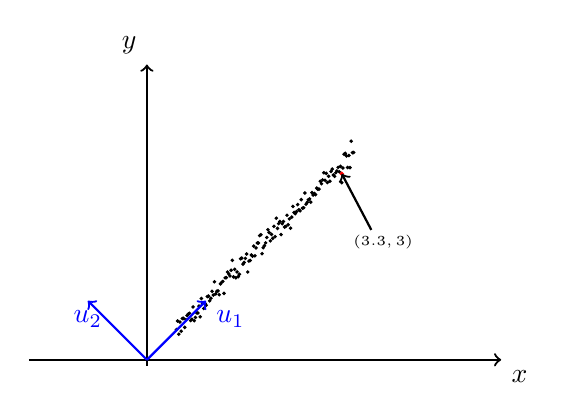
\begin{tikzpicture}[scale=0.75]
  \foreach \x/\y in {0.5/0.511870677093,0.520134228188/0.657474112041,0.540268456376/0.433301054831,0.560402684564/0.639402738784,0.580536912752/0.484888418032,0.60067114094/0.698401610126,0.620805369128/0.7012649978,0.640939597315/0.550258599782,0.661073825503/0.678863257247,0.681208053691/0.75063942818,0.701342281879/0.776722844493,0.721476510067/0.787974629261,0.741610738255/0.664867942136,0.761744966443/0.686496368534,0.781879194631/0.895235993285,0.802013422819/0.661601738133,0.822147651007/0.717376222072,0.842281879195/0.796219038444,0.862416107383/0.792290066926,0.88255033557/0.908555964509,0.902684563758/0.728213610997,0.922818791946/1.03682525621,0.942953020134/0.959254604949,0.963087248322/0.868395203865,0.98322147651/0.954903379431,1.0033557047/0.925500701421,1.02348993289/1.0700072327,1.04362416107/1.07910784654,1.06375838926/0.998680883498,1.08389261745/1.04215184899,1.10402684564/1.15961695354,1.12416107383/1.09641078989,1.14429530201/1.32135817413,1.1644295302/1.11554678055,1.18456375839/1.15881333579,1.20469798658/1.16650720076,1.22483221477/1.10170000196,1.24496644295/1.2856802819,1.26510067114/1.31032588214,1.28523489933/1.32664087434,1.30536912752/1.12586374789,1.3255033557/1.38744778116,1.34563758389/1.39149477354,1.36577181208/1.4858410387,1.38590604027/1.45489220706,1.40604026846/1.42066727608,1.42617449664/1.51638552543,1.44630872483/1.68453235672,1.46644295302/1.40404774902,1.48657718121/1.53217972768,1.5067114094/1.38840003053,1.52684563758/1.48738732887,1.54697986577/1.40903699426,1.56711409396/1.44846302024,1.58724832215/1.71184821717,1.60738255034/1.72156284303,1.62751677852/1.62088209802,1.64765100671/1.64829634188,1.6677852349/1.71789690662,1.68791946309/1.79158703578,1.70805369128/1.4865801932,1.72818791946/1.67235453921,1.74832214765/1.68309131722,1.76845637584/1.77403777092,1.78859060403/1.75540229337,1.80872483221/1.92421819935,1.8288590604/1.76070413373,1.84899328859/1.89440714397,1.86912751678/1.97867095812,1.88926174497/1.9767064361,1.90939597315/2.10350092601,1.92953020134/2.11726782381,1.94966442953/1.79668775603,1.96979865772/1.8979484069,1.98993288591/1.93277217634,2.01006711409/1.97986856224,2.03020134228/2.07115112966,2.05033557047/2.20256198706,2.07046979866/2.15486115796,2.09060402685/2.0135265175,2.11073825503/2.12456025274,2.13087248322/2.05492034879,2.15100671141/2.26017076362,2.1711409396/2.08564641805,2.19127516779/2.39746927122,2.21140939597/2.22522490056,2.23154362416/2.30668911212,2.25167785235/2.3405336089,2.27181208054/2.12057378128,2.29194630872/2.30428172148,2.31208053691/2.34209297556,2.3322147651/2.24731114226,2.35234899329/2.25863238242,2.37248322148/2.44749889836,2.39261744966/2.28794979535,2.41275167785/2.38637728425,2.43288590604/2.22855717892,2.45302013423/2.41476899048,2.47315436242/2.59725934406,2.4932885906/2.49509909292,2.51342281879/2.475381467,2.53355704698/2.50849761644,2.55369127517/2.62894898586,2.57382550336/2.53964404005,2.59395973154/2.52304084678,2.61409395973/2.71120042668,2.63422818792/2.56659063768,2.65436241611/2.57507058482,2.6744966443/2.82455379784,2.69463087248/2.63449675455,2.71476510067/2.66520230501,2.73489932886/2.70961994446,2.75503355705/2.72467839298,2.77516778523/2.67053791754,2.79530201342/2.83185765234,2.81543624161/2.79124434869,2.8355704698/2.81620859231,2.85570469799/2.79664069335,2.87583892617/2.90595671478,2.89597315436/2.88803599738,2.91610738255/2.89044757658,2.93624161074/3.02268962114,2.95637583893/2.98120872379,2.97651006711/3.04538380829,2.9966442953/3.16677251227,3.01677852349/3.03954291368,3.03691275168/3.15577291285,3.05704697987/3.00237643869,3.07718120805/3.10771652408,3.09731543624/3.02357015434,3.11744966443/3.18830966895,3.13758389262/3.22886917638,3.15771812081/3.12806798086,3.17785234899/3.10674403454,3.19798657718/3.16730762796,3.21812080537/3.19780291521,3.23825503356/3.25800939012,3.25838926174/3.18329683084,3.27852348993/3.27555040698,3.3/3,3.31879194631/3.24878603874,3.3389261745/3.48010644439,3.35906040268/3.49488774085,3.37919463087/3.45169839488,3.39932885906/3.2562776487,3.41946308725/3.45982610179,3.43959731544/3.25489013156,3.45973154362/3.70199350258,3.47986577181/3.50720556225,3.5/3.51067497333}
    {
      \node at (\x,\y)[circle,draw=black,fill=black,inner sep=0pt,minimum size=0.3mm]{};
    }
  \onslide<3->{
    \node (A) at (3.3,3.15)[circle,draw=red,fill=red,inner sep=0pt,minimum size=0.4mm]{};
    \node at (4,2) {\tiny{$(3.3,3)$}};
    \draw [thick, black, ->] (3.8,2.2) -- (3.3,3.15) ;}
  \draw [thick, black, ->] (-2,0) -- (6, 0)node[anchor=north west] {$x$};
  \draw [thick, black, ->] (0,-0.1) -- (0, 5)node[anchor=south east] {$y$};
  \draw [thick,blue,->] (0,0) -- (1,1)node [anchor=north west]{$u_1$};
  \draw [thick,blue,->] (0,0) -- (-1,1)node[anchor=north ]{$u_2$};
\end{tikzpicture}
}

% Slide 37
\begin{frame}
  \myheading{Module 6.5 : PCA : Interpretation 2}
\end{frame}

%----------------------------------------------------------------------------------------------------------
% Slide 38
\begin{frame}
  \begin{overlayarea}{\textwidth}{\textheight}
    \onslide<1->{
      Given $n$ orthogonal linearly independent vectors $P=p_1,p_2,\cdots,p_n$ we can represent $x_i$ exactly as a linear combination of these vectors.
    }
    \onslide<2->{
      \begin{equation*}
        x_i= \sum_{j=1}^{n} \alpha_{ij} p_j \hspace{0.3cm}[\textnormal{we know how to estimate $\alpha_{ij}'s$ but we will come back to that later}]
      \end{equation*}
    }
    \onslide<3->{But we are interested only in the top-k dimensions (we want to get rid of noisy \& redundant dimensions)
      \begin{equation*}
        \hat{x}_i = \sum_{j=1}^{k} \alpha_{ik} p_k
      \end{equation*}
    }
    \onslide<4->{
      We want to select $p_{i}'s$ such that we minimise the reconstructed error
      \begin{equation*}
        e= \sum_{i=1}^{m} (x_i - \hat{x}_i)^T (x_i - \hat{x}_i)
      \end{equation*}
    }
  \end{overlayarea}
\end{frame}


%----------------------------------------------------------------------------------------------------------
% Slide 39
\begin{frame}[shrink=20]%change this to change the font
  \begin{columns}
    \column{0.5\textwidth}
    \begin{overlayarea}{\textwidth}{\textheight}
      \begin{align*}
          \onslide<1->{  e &= \sum_{i=1}^{m} (x_i - \hat{x}_i)^T (x_i - \hat{x}_i) } \\
          \onslide<2->{
            &= \sum_{i=1}^{m} \left(\sum_{j=1}^{n} \alpha_{ij}p_j - \sum_{j=1}^{k} \alpha_{ij} p_j\right)^2} \\
          \onslide<3->{ &= \sum_{i=1}^{m} \left(\sum_{j=k+1}^{n}\alpha_{ij}p_j\right)^2 = \sum_{i=1}^{m} \left(\sum_{j=k+1}^{n}\alpha_{ij}p_j\right)^T\left(\sum_{j=k+1}^{n}\alpha_{ij}p_j\right)} \\
          \onslide<4->{ &= \sum_{i=1}^{m} \left(\alpha_{i,k+1}p_{k+1}+\alpha_{i,k+2}p_{k+2}+\hdots+\alpha_{i,n}p_n\right)^T\left(\alpha_{i,k+1}p_{k+1}+\alpha_{i,k+2}p_{k+2}+\hdots+\alpha_{i,n}p_n\right)} \\
          \onslide<5->{ &= \sum_{i=1}^{m} \sum_{j=k+1}^{n} \alpha_{ij}p_j^T p_j \alpha_{ij} + \sum_{i=1}^{m} \sum_{j=k+1}^{n} \sum_{L=k+1,L\neq k}^{n} \alpha_{ij}p_j^T p_L \alpha_{iL}} \\
          \onslide<6->{&= \sum_{i=1}^{m} \sum_{j=k+1}^{n} \alpha_{ij}^2 \qquad \qquad (\because p_j^T p_j =1, p_i^T p_j =0 \quad \forall i\neq j) }\\
          \onslide<7->{&= \sum_{i=1}^{m} \sum_{j=k+1}^{n} \left(x_i^T p_j\right)^2 } \\
      \end{align*}
    \end{overlayarea}
    \column{0.5\textwidth}
    \begin{overlayarea}{\textwidth}{\textheight}
      \begin{tabular}{|l}
        {$\begin{aligned}
              \onslide<8->{&= \sum_{i=1}^{m} \sum_{j=k+1}^{n} \left(p_j^T x_i\right)\left(x_i^T p_j\right)} \\
              \onslide<9->{&= \sum_{j=k+1}^{n} p_j^T \left( \sum_{i=1}^{m} x_i x_i^T\right) p_j  } \\
              \onslide<10->{ &= \sum_{j=k+1}^{n} p_j^T m C p_j \qquad \left[\because \frac{1}{m} \sum_{i=1}^{m} x_i x_i^T = \frac{X^TX}{m} = C\right]}
          \end{aligned}$}
      \end{tabular}
    \end{overlayarea}
  \end{columns}
\end{frame}

%----------------------------------------------------------------------------------------------------------
% Slide 40
\begin{frame}
  \begin{overlayarea}{\textwidth}{\textheight}
    \onslide<1->{
      \vspace{1.3cm}

      We want to minimize $e$
      \begin{equation*}
        \min_{p_{k+1},p_{k+2},\cdots,p_{n}} \sum_{j=k+1}^{n} p_j^T m C p_j \qquad s.t.\quad p_j^Tp_j =1 \quad \forall j = k+1,k+2,\cdots,n
      \end{equation*}

    }
    \onslide<2->{
      The solution to the above problem is given by the eigen vectors corresponding to the smallest eigen values of $C$ (\textbf{Proof : refer Slide 26}). }

    \onslide<3->{
      \vspace{0.7cm}
      Thus we select $P=p_1,p_2,\cdots,p_n$ as eigen vectors of $C$ and retain only top-k eigen vectors to express the data [or discard the eigen vectors $k+1,\cdots,n$]
    }
  \end{overlayarea}
\end{frame}

%----------------------------------------------------------------------------------------------------------
% Slide 41
\begin{frame}
  %\begin{overlayarea}{\textwidth}{\textheight}
  %\begin{center}
  \begin{block}{Key Idea}
    Minimize the error in reconstructing $x_i$ after projecting the data on to a new basis.
  \end{block}
  %\end{center}
  %\end{overlayarea}
\end{frame}

%----------------------------------------------------------------------------------------------------------
% Slide 42
\begin{frame}
  \begin{center}
    \textit{Let's look at the \textbf{`Reconstruction Error'} in the context of our toy example}
  \end{center}
\end{frame}

%----------------------------------------------------------------------------------------------------------
% Slide 43
\begin{frame}
  \begin{columns}
    \column{0.5\textwidth}<1->
    \begin{overlayarea}{\textwidth}{\textheight}
      \makebox[\textwidth][c]{\usebox{\pcareconstructioncontent}}
      % 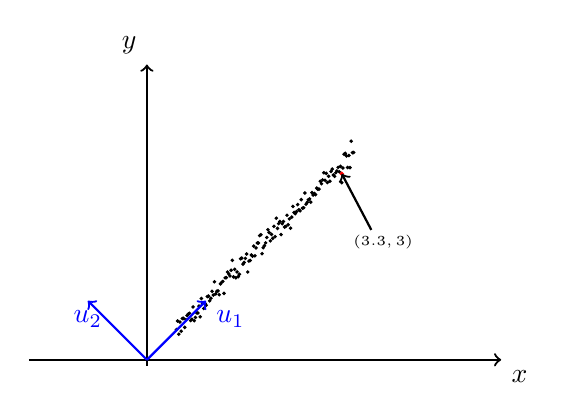
\begin{tikzpicture}[scale=0.75]
  \foreach \x/\y in {0.5/0.511870677093,0.520134228188/0.657474112041,0.540268456376/0.433301054831,0.560402684564/0.639402738784,0.580536912752/0.484888418032,0.60067114094/0.698401610126,0.620805369128/0.7012649978,0.640939597315/0.550258599782,0.661073825503/0.678863257247,0.681208053691/0.75063942818,0.701342281879/0.776722844493,0.721476510067/0.787974629261,0.741610738255/0.664867942136,0.761744966443/0.686496368534,0.781879194631/0.895235993285,0.802013422819/0.661601738133,0.822147651007/0.717376222072,0.842281879195/0.796219038444,0.862416107383/0.792290066926,0.88255033557/0.908555964509,0.902684563758/0.728213610997,0.922818791946/1.03682525621,0.942953020134/0.959254604949,0.963087248322/0.868395203865,0.98322147651/0.954903379431,1.0033557047/0.925500701421,1.02348993289/1.0700072327,1.04362416107/1.07910784654,1.06375838926/0.998680883498,1.08389261745/1.04215184899,1.10402684564/1.15961695354,1.12416107383/1.09641078989,1.14429530201/1.32135817413,1.1644295302/1.11554678055,1.18456375839/1.15881333579,1.20469798658/1.16650720076,1.22483221477/1.10170000196,1.24496644295/1.2856802819,1.26510067114/1.31032588214,1.28523489933/1.32664087434,1.30536912752/1.12586374789,1.3255033557/1.38744778116,1.34563758389/1.39149477354,1.36577181208/1.4858410387,1.38590604027/1.45489220706,1.40604026846/1.42066727608,1.42617449664/1.51638552543,1.44630872483/1.68453235672,1.46644295302/1.40404774902,1.48657718121/1.53217972768,1.5067114094/1.38840003053,1.52684563758/1.48738732887,1.54697986577/1.40903699426,1.56711409396/1.44846302024,1.58724832215/1.71184821717,1.60738255034/1.72156284303,1.62751677852/1.62088209802,1.64765100671/1.64829634188,1.6677852349/1.71789690662,1.68791946309/1.79158703578,1.70805369128/1.4865801932,1.72818791946/1.67235453921,1.74832214765/1.68309131722,1.76845637584/1.77403777092,1.78859060403/1.75540229337,1.80872483221/1.92421819935,1.8288590604/1.76070413373,1.84899328859/1.89440714397,1.86912751678/1.97867095812,1.88926174497/1.9767064361,1.90939597315/2.10350092601,1.92953020134/2.11726782381,1.94966442953/1.79668775603,1.96979865772/1.8979484069,1.98993288591/1.93277217634,2.01006711409/1.97986856224,2.03020134228/2.07115112966,2.05033557047/2.20256198706,2.07046979866/2.15486115796,2.09060402685/2.0135265175,2.11073825503/2.12456025274,2.13087248322/2.05492034879,2.15100671141/2.26017076362,2.1711409396/2.08564641805,2.19127516779/2.39746927122,2.21140939597/2.22522490056,2.23154362416/2.30668911212,2.25167785235/2.3405336089,2.27181208054/2.12057378128,2.29194630872/2.30428172148,2.31208053691/2.34209297556,2.3322147651/2.24731114226,2.35234899329/2.25863238242,2.37248322148/2.44749889836,2.39261744966/2.28794979535,2.41275167785/2.38637728425,2.43288590604/2.22855717892,2.45302013423/2.41476899048,2.47315436242/2.59725934406,2.4932885906/2.49509909292,2.51342281879/2.475381467,2.53355704698/2.50849761644,2.55369127517/2.62894898586,2.57382550336/2.53964404005,2.59395973154/2.52304084678,2.61409395973/2.71120042668,2.63422818792/2.56659063768,2.65436241611/2.57507058482,2.6744966443/2.82455379784,2.69463087248/2.63449675455,2.71476510067/2.66520230501,2.73489932886/2.70961994446,2.75503355705/2.72467839298,2.77516778523/2.67053791754,2.79530201342/2.83185765234,2.81543624161/2.79124434869,2.8355704698/2.81620859231,2.85570469799/2.79664069335,2.87583892617/2.90595671478,2.89597315436/2.88803599738,2.91610738255/2.89044757658,2.93624161074/3.02268962114,2.95637583893/2.98120872379,2.97651006711/3.04538380829,2.9966442953/3.16677251227,3.01677852349/3.03954291368,3.03691275168/3.15577291285,3.05704697987/3.00237643869,3.07718120805/3.10771652408,3.09731543624/3.02357015434,3.11744966443/3.18830966895,3.13758389262/3.22886917638,3.15771812081/3.12806798086,3.17785234899/3.10674403454,3.19798657718/3.16730762796,3.21812080537/3.19780291521,3.23825503356/3.25800939012,3.25838926174/3.18329683084,3.27852348993/3.27555040698,3.3/3,3.31879194631/3.24878603874,3.3389261745/3.48010644439,3.35906040268/3.49488774085,3.37919463087/3.45169839488,3.39932885906/3.2562776487,3.41946308725/3.45982610179,3.43959731544/3.25489013156,3.45973154362/3.70199350258,3.47986577181/3.50720556225,3.5/3.51067497333}
    {
      \node at (\x,\y)[circle,draw=black,fill=black,inner sep=0pt,minimum size=0.3mm]{};
    }
  \onslide<3->{
    \node (A) at (3.3,3.15)[circle,draw=red,fill=red,inner sep=0pt,minimum size=0.4mm]{};
    \node at (4,2) {\tiny{$(3.3,3)$}};
    \draw [thick, black, ->] (3.8,2.2) -- (3.3,3.15) ;}
  \draw [thick, black, ->] (-2,0) -- (6, 0)node[anchor=north west] {$x$};
  \draw [thick, black, ->] (0,-0.1) -- (0, 5)node[anchor=south east] {$y$};
  \draw [thick,blue,->] (0,0) -- (1,1)node [anchor=north west]{$u_1$};
  \draw [thick,blue,->] (0,0) -- (-1,1)node[anchor=north ]{$u_2$};
\end{tikzpicture}

      \begin{itemize}\justifying
        \item<1-> $u_1=[1,1]$ and $u_2=[-1,1]$ are the new basis vectors
        \item<2-> Let us convert them to unit vectors $u_1=\begin{bmatrix}
                  \frac{1}{\sqrt{2}} & \frac{1}{\sqrt{2}}
                \end{bmatrix}$
              \& $u_2=\begin{bmatrix}
                  \frac{-1}{\sqrt{2}} & \frac{1}{\sqrt{2}}
                \end{bmatrix}$


      \end{itemize}
    \end{overlayarea}

    \column{0.5\textwidth}<3->
    \begin{overlayarea}{\textwidth}{\textheight}
      \begin{itemize}\justifying
        \item<3-> Consider the point $x=[3.3,3]$ in the original data
        \item<4-> $\alpha_1 = x^Tu_1= {6.3}/{\sqrt{2}}$ \\
              $\alpha_2 = x^Tu_2= {0.3}/{\sqrt{2}}$
        \item<5-> the perfect reconstruction of $x$ is given by (using $n=2$ dimensions)
              \begin{equation*}
                x= \alpha_1 u_1 + \alpha_2 u_2 = \begin{bmatrix}3.3 & 3 \end{bmatrix}
              \end{equation*}
        \item<6-> But we are going to reconstruct it using fewer (only $k=1<n$ dimensions, ignoring the low variance $u_2$ dimension)
              \begin{equation*}
                \hat{x}=\alpha_1 u_1=\begin{bmatrix}3.15 & 3.15 \end{bmatrix}
              \end{equation*}
              (reconstruction with minimum error)
      \end{itemize}
    \end{overlayarea}
  \end{columns}
\end{frame}

%----------------------------------------------------------------------------------------------------------
% Slide 44
\begin{frame}
  \begin{overlayarea}{\textwidth}{\textheight}
    \begin{block}{Recap}
      \begin{itemize}\justifying
        \item<1-> The eigen vectors of a matrix with distinct eigenvalues are linearly independent
        \item<2-> The eigen vectors of a square symmetric matrix are orthogonal
        \item<3-> PCA exploits this fact by representing the data using a new basis comprising only the top-$k$ eigen vectors
        \item<4-> The $n-k$ dimensions which contribute very little to the reconstruction error are discarded
        \item<5-> \textbf{These are also the directions along which the variance is minimum}
      \end{itemize}
    \end{block}
  \end{overlayarea}
\end{frame}
